%----------------------------------------------------------------------------------------
%	PACKAGES AND OTHER DOCUMENT CONFIGURATIONS
%----------------------------------------------------------------------------------------

\documentclass{article}

\usepackage{fancyhdr} % Required for custom headers
\usepackage{lastpage} % Required to determine the last page for the footer
\usepackage{extramarks} % Required for headers and footers
\usepackage[usenames,dvipsnames]{color} % Required for custom colors
\usepackage{pgf} % Required to insert pgf plots from matplotlib
\usepackage{graphicx} % Required to insert images
\usepackage{listings} % Required for insertion of code
\usepackage{courier} % Required for the courier font
\usepackage{lipsum} % Used for inserting dummy 'Lorem ipsum' text into the template
\usepackage[utf8]{inputenc}
\usepackage[ngerman]{babel}
\usepackage{subcaption, caption, tabularx, minted}
\usepackage{hyperref}

% Margins
\topmargin=-0.45in
\evensidemargin=0in
\oddsidemargin=0in
\textwidth=6.5in
\textheight=9.0in
\headsep=0.25in

\linespread{1.1} % Line spacing

% Set up the header and footer
\pagestyle{fancy}
%\lhead{\hmwkAuthorName} % Top left header
\chead{\hmwkClass\ : \hmwkTitle} % Top center head
\rhead{\firstxmark} % Top right header
\lfoot{\lastxmark} % Bottom left footer
\cfoot{} % Bottom center footer
\rfoot{Page\ \thepage\ of\ \protect\pageref{LastPage}} % Bottom right footer
\renewcommand\headrulewidth{0.4pt} % Size of the header rule
\renewcommand\footrulewidth{0.4pt} % Size of the footer rule

\setlength\parindent{0pt} % Removes all indentation from paragraphs

%----------------------------------------------------------------------------------------
%	CODE INCLUSION CONFIGURATION
%----------------------------------------------------------------------------------------

\definecolor{MyDarkGreen}{rgb}{0.0,0.4,0.0} % This is the color used for comments
\lstloadlanguages{Perl} % Load Perl syntax for listings, for a list of other languages supported see: ftp://ftp.tex.ac.uk/tex-archive/macros/latex/contrib/listings/listings.pdf
\lstset{language=Perl, % Use Perl in this example
        frame=single, % Single frame around code
        basicstyle=\small\ttfamily, % Use small true type font
        keywordstyle=[1]\color{Blue}\bf, % Perl functions bold and blue
        keywordstyle=[2]\color{Purple}, % Perl function arguments purple
        keywordstyle=[3]\color{Blue}\underbar, % Custom functions underlined and blue
        identifierstyle=, % Nothing special about identifiers                                         
        commentstyle=\usefont{T1}{pcr}{m}{sl}\color{MyDarkGreen}\small, % Comments small dark green courier font
        stringstyle=\color{Purple}, % Strings are purple
        showstringspaces=false, % Don't put marks in string spaces
        tabsize=5, % 5 spaces per tab
        %
        % Put standard Perl functions not included in the default language here
        morekeywords={rand},
        %
        % Put Perl function parameters here
        morekeywords=[2]{on, off, interp},
        %
        % Put user defined functions here
        morekeywords=[3]{test},
       	%
        morecomment=[l][\color{Blue}]{...}, % Line continuation (...) like blue comment
        numbers=left, % Line numbers on left
        firstnumber=1, % Line numbers start with line 1
        numberstyle=\tiny\color{Blue}, % Line numbers are blue and small
        stepnumber=5 % Line numbers go in steps of 5
}

% Creates a new command to include a perl script, the first parameter is the filename of the script (without .pl), the second parameter is the caption
\newcommand{\perlscript}[2]{
\begin{itemize}
\item[]\lstinputlisting[caption=#2,label=#1]{#1.pl}
\end{itemize}
}

%----------------------------------------------------------------------------------------
%	DOCUMENT STRUCTURE COMMANDS
%	Skip this unless you know what you're doing
%----------------------------------------------------------------------------------------

% Header and footer for when a page split occurs within a problem environment
\newcommand{\enterProblemHeader}[1]{
%\nobreak\extramarks{#1}{#1 continued on next page\ldots}\nobreak
%\nobreak\extramarks{#1 (continued)}{#1 continued on next page\ldots}\nobreak
}

% Header and footer for when a page split occurs between problem environments
\newcommand{\exitProblemHeader}[1]{
%\nobreak\extramarks{#1 (continued)}{#1 continued on next page\ldots}\nobreak
%\nobreak\extramarks{#1}{}\nobreak
}

\setcounter{secnumdepth}{0} % Removes default section numbers
\newcounter{homeworkProblemCounter} % Creates a counter to keep track of the number of problems

\newcommand{\homeworkProblemName}{}
\newenvironment{homeworkProblem}[1][Problem \arabic{homeworkProblemCounter}]{ % Makes a new environment called homeworkProblem which takes 1 argument (custom name) but the default is "Problem #"
\stepcounter{homeworkProblemCounter} % Increase counter for number of problems
\renewcommand{\homeworkProblemName}{#1} % Assign \homeworkProblemName the name of the problem
\section{\homeworkProblemName} % Make a section in the document with the custom problem count
%\enterProblemHeader{\homeworkProblemName} % Header and footer within the environment
}{
%\exitProblemHeader{\homeworkProblemName} % Header and footer after the environment
}

\newcommand{\problemAnswer}[1]{ % Defines the problem answer command with the content as the only argument
\noindent\framebox[\columnwidth][c]{\begin{minipage}{0.98\columnwidth}#1\end{minipage}} % Makes the box around the problem answer and puts the content inside
}

\newcommand{\homeworkSectionName}{}
\newenvironment{homeworkSection}[1]{ % New environment for sections within homework problems, takes 1 argument - the name of the section
\renewcommand{\homeworkSectionName}{#1} % Assign \homeworkSectionName to the name of the section from the environment argument
\subsection{\homeworkSectionName} % Make a subsection with the custom name of the subsection
%\enterProblemHeader{\homeworkProblemName\ [\homeworkSectionName]} % Header and footer within the environment
}{
%\enterProblemHeader{\homeworkProblemName} % Header and footer after the environment
}

%----------------------------------------------------------------------------------------
%	NAME AND CLASS SECTION
%----------------------------------------------------------------------------------------

\newcommand{\hmwkTitle}{Exercise\ \#8} % Assignment title
\newcommand{\hmwkDueDate}{Tuesday,\ June 16,\ 2015} % Due date
\newcommand{\hmwkClass}{Advanced Parallel Computing} % Course/class
\newcommand{\hmwkClassTime}{} % Class/lecture time
\newcommand{\hmwkClassInstructor}{} % Teacher/lecturer
\newcommand{\hmwkAuthorName}{Svend Dorkenwald, Günther Schindler} % Your name

%----------------------------------------------------------------------------------------
%	TITLE PAGE
%----------------------------------------------------------------------------------------

\title{
\vspace{2in}
\textmd{\textbf{\hmwkClass:\ \hmwkTitle}}\\
\normalsize\vspace{0.1in}\small{Due\ on\ \hmwkDueDate}\\
\vspace{0.1in}\large{\textit{\hmwkClassTime}}
\vspace{3in}
}

\author{\textbf{\hmwkAuthorName}}
\date{} % Insert date here if you want it to appear below your name

%----------------------------------------------------------------------------------------

\begin{document}

\maketitle

%----------------------------------------------------------------------------------------
%	TABLE OF CONTENTS
%----------------------------------------------------------------------------------------

%\setcounter{tocdepth}{1} % Uncomment this line if you don't want subsections listed in the ToC

\newpage
%\tableofcontents
\newpage

%----------------------------------------------------------------------------------------
%	Reading
%----------------------------------------------------------------------------------------

\begin{homeworkProblem}[Reading]
\subsection{The AMD Opteron Northbridge Architecture}
The authors introduce the upcoming Northbridge Architecture from AMD. Therefore, they discuss the latest features and present numbers supporting the abilities of thi chip. \\
Their new design is all about increasing bandwidth and while keeping the latency at a low level. They manage to do this by adding one extra hyperTransport port which clocks at the same frequency as one core. Compared to older generations their Cores are now connected by Direct Connect allowing bandwidths of 8 Gbytes/s between any neighbouring component. Finally, they optimized their system with regard to latency for one-, two-, and four-node systems. \\
Unfortunately, the authors do not manage to either proof the capabilities of their chip by comparing it to a latest Intel chip nor are they able to introduce anything brand-new. This paper seems like an update on the latest developments at AMD and includes a surprisingly large part about their future plans. Hence, we reject this paper (strongly!).



\subsection{The SGI Origin: a ccNUMA highly scalableserver}
This paper introduces the 'SGI Origin 2000', a cache-coherent non-uniform memory access
multiprocessor, which is scaling to small and large processor counts without any bandwidth,
latency, or cost cliffs. It uses the distributed shared memory architecture with a crossbar
based I/O subsystem. The basic building block of the Origin system is the dual-processor
node with 4 GB of main memory. The architecture supports up to 512 nodes, for a maximum
configuration of 1024 processors and 1 TB of main memory. A non-blocking bristled fat
hypercube network is used to provide a high bisection bandwidth with low latency to local
and remote memory. Origin also includes several features to help the performance of 
applications including hardware and software support for page migration and fast
synchronization.
\\
The introduced architecture surprised us with its good scalability and performance results.
We think that the use of distributed shared memory combined with the cache-coherent 
processors leads to a highly productivity from programmer perspective. The support for 
page migration and fast synchronization is also a plus for most applications. Therefor, we
strongly accept this paper.
\end{homeworkProblem}

%----------------------------------------------------------------------------------------
%	Red-Black Tree – Coarse grain locking
%----------------------------------------------------------------------------------------

\begin{homeworkProblem}[Red-Black Tree – Coarse grain locking]
Our coarse grain locking is based on a shared read lock and a exclusive write lock. We
implemented the lock using the PThread reader-writer-lock which allows:
\begin{itemize}
\item Any number of threads hold a reader lock at the same time
\item Only one thread may hold a writer lock
\item When a thread holds a writer lock no reader locks are held by any other thread
\end{itemize}
If we performe a search-operation, we simply lock this section shared so any other thread
can search concurrent.
\begin{lstlisting}{c}
void* rbtree_lookup() {
    /* Shared lock */
    pthread_rwlock_rdlock(&rwlock);
    ...
    /* Unlock */
    pthread_rwlock_unlock(&rwlock);
}
\end{lstlisting}
If we performe a add-operation, we lock the whole tree so no other thread can search or
add concurrent.
\begin{lstlisting}{c}
void rbtree_insert() {
    /* Lock the whole tree */
    pthread_rwlock_wrlock(&rwlock);
    ...
    /* Unlock the tree */
    pthread_rwlock_unlock(&rwlock);
}
\end{lstlisting}

\end{homeworkProblem}

%----------------------------------------------------------------------------------------
%	Red-Black Tree – Performance of coarse-grain locking
%----------------------------------------------------------------------------------------

\begin{homeworkProblem}[Red-Black Tree – Performance of coarse-grain locking]
The performance analysis of our parallel implementation show quite bad results. We don't
reache nearly the performance of our sequential implementation. This is not surprising, if
we consider that only one thread at a time is able to performe an add-operation, whereas all 
other threads spin on the lock and do nothing. Due to that, the parallel implementation will
be performed sequential with additional overhead for parallelisation and lock-spinning.
\begin{center}
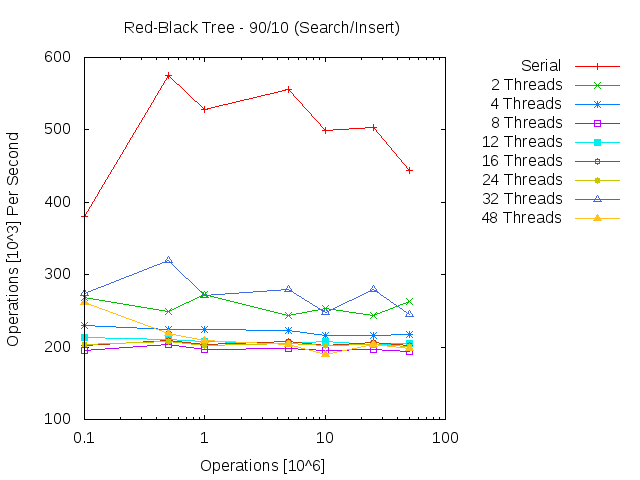
\includegraphics[width=0.7\columnwidth]{update_rate_90_10.png}
\end{center}
Surprisingly, we get the best results for a ratio of 90/10 with a thread count of 2 and 32.
All other thread counts seem to be quite equal.
\begin{center}
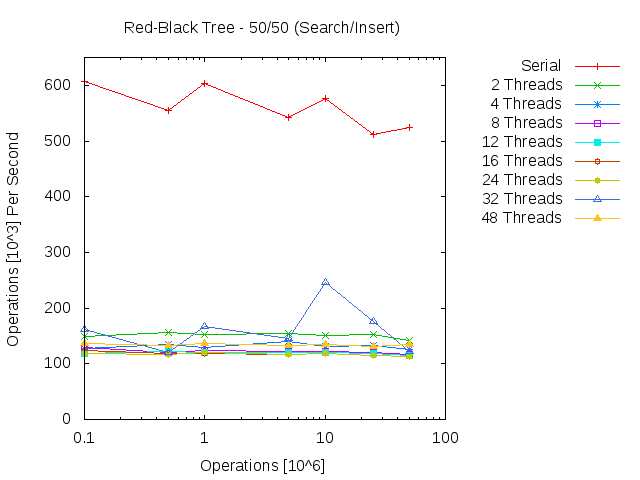
\includegraphics[width=0.7\columnwidth]{update_rate_50_50.png}
\end{center}
With increasing add-operation, the sequential part becomes bigger and it doesn't matter how
many threads we use.
\begin{center}
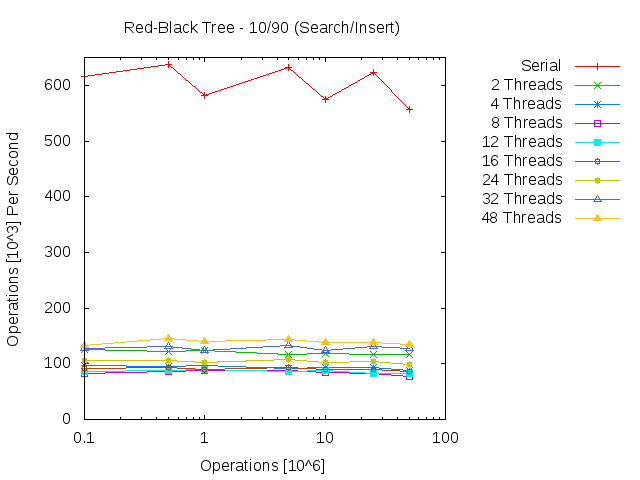
\includegraphics[width=0.7\columnwidth]{update_rate_10_90.png}
\end{center}
The only adventage of the parallel implementation seems to be the good scalability, since we
don't get performance losses with increasing operation numbers.
\end{homeworkProblem}

%----------------------------------------------------------------------------------------
%	Red-Black Tree – Considerations for fine-grain Locking
%----------------------------------------------------------------------------------------
\begin{homeworkProblem}[Red-Black Tree – Considerations for fine-grain Locking]
The basic idea of our fine-grain locking considerations is to store a lock in each node
so we can lock only certain parts of the tree. If we performe a search operation we would
simply read-lock every involved node, which allows us to search concurrent and ensure 
correctness of the data.
\\
When inserting a new value it is going to be a little more complicated. In our implementation,
we first insert a new node into the tree as we would into an ordinary binary search tree.
So far we would just need to read-lock as long as we find the right place and then 
write-lock the destination node. The problem is that the resulting tree may not satify our 
five red-black tree properties, so we call to insert\_case1() function which begins the 
process of correcting the tree so that it satifies the properties once more.
\\
Our five insert cases need to access and modify the parent-, grandparent-, uncle-, left- and
right-node like in the picture shown below.
\begin{center}
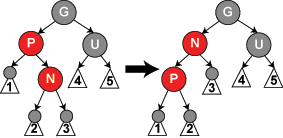
\includegraphics[width=0.5\columnwidth]{Red-black.png}
\end{center}
\end{homeworkProblem}
Thus, we could implement a function which write-locks the whole family which is called if 
we call our insert\_case functions. In the case of an insert conflict only one thread can
access this family nodes whereas the others spin.
\\
A huge disadvantage of this implementation would be the big memory amount which is needed
to store a lock in each node. Also, there will be spent a lot of time with lock creation
and spinning, but the amount of concurrency should strongly increase.
\clearpage
\end{document}
